\chapter{Mission}
\section{Sujet de stage}
Le sujet de mon stage était initialement \texttt{Développement/Intégration de fonctions de Vision par ordinateur pour l’inspection automatisée}. Durant toute la période de mon stage, mon travail s'est axé autour d'un logiciel appelé \texttt{PowerEye}. \texttt{PowerEye} est un logiciel développé pour des scénarios industriels qui utilise la vision par ordinateur pour détecter les défauts des pièces sur la chaîne de production. Les laboratoires de l’UTC faisant partie de ce projet, ils assurent le développement des machines apprenantes. Deltacad est responsable de la conception de l'interface de l'ensemble du projet et de l'intégration des autres fonctions. \\

Avant que je ne commence mon stage, \texttt{PowerEye} avait déjà été conçu avec certaines fonctionnalités ainsi qu'un prototype d'interface. Cependant, il était clair que le système n'était pas encore adapté à une application formelle au sein de l'entreprise. Par conséquent, la tâche principale de mon stage consistait à concevoir et améliorer une interface homme-machine plus pratique basée sur le prototype de l'interface et essayer de tester les pièces d'AML Systems\footnote{un société du segment éclairage du groupe Johnson Electric, conçoit, produit et commercialise, des solutions pour améliorer la visibilité, la sécurité, et le confort du conducteur} à l'aide de cette interface après intégration de la fonction.\\

En ce qui concerne les lignes directrices spécifiques pour la conception de l'interface, le chef de projet et le suiveur m'ont fourni un aperçu général des différents modules qu'elle contiendrait et des fonctionnalités qu'elle pourrait inclure. Après avoir confirmé le thème et le programme de travail, mon stage a officiellement commencé.\\

\newpage
\section{Planning de stage}
Au début de mon stage, mes tâches étaient planifiées en trois phases : 
\begin{itemize}
    \item \textbf{1. }Développement de l'interface homme-machine de PowerEye 
    \item \textbf{2. }Test sur les données de l'entreprise partenaire AML système
    \item \textbf{3. }Déploiement d'applications dans le système AML
\end{itemize}

Dans le cadre du travail réel, pour chaque phase de la tâche, je l'ai décomposée en différentes étapes. 


\newpage
\section{Contributions}
Comme mentionné dans la section précédente, lorsque j'ai commencé à travailler sur le projet, il existait déjà un prototype d'interface ainsi que certains modules fonctionnels.
\begin{figure}[H]
    \centering
    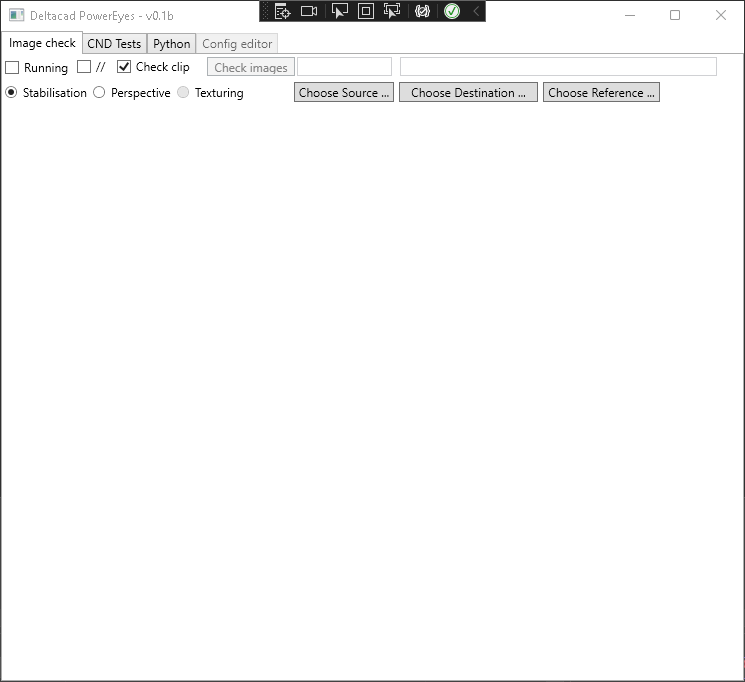
\includegraphics[height=5cm]{ressources/images/prototype.png}
    \caption{Prototype d'interface PowerEye}
\end{figure}
L'interface se compose de quatre modules: Image check, CND Tests, python et config editor. Il contient des méthodes d'application de de Template Matching pour la détection des pièces et des modèles d'entraînement pour les tests avec des ensembles de données.\\
Mais le fait est que l'interface prototype n'est pas suffisante pour inclure toutes les fonctionnalités envisagées par PowerEye. Par conséquent, ma principale contribution tout au long du stage a été la conception et le développement d'une nouvelle version de l'interface \texttt{PowerEye}. À la fin du stage, la nouvelle version de l'interface de powereye ressemblait à ceci. \\
\begin{figure}[H]
    \centering
    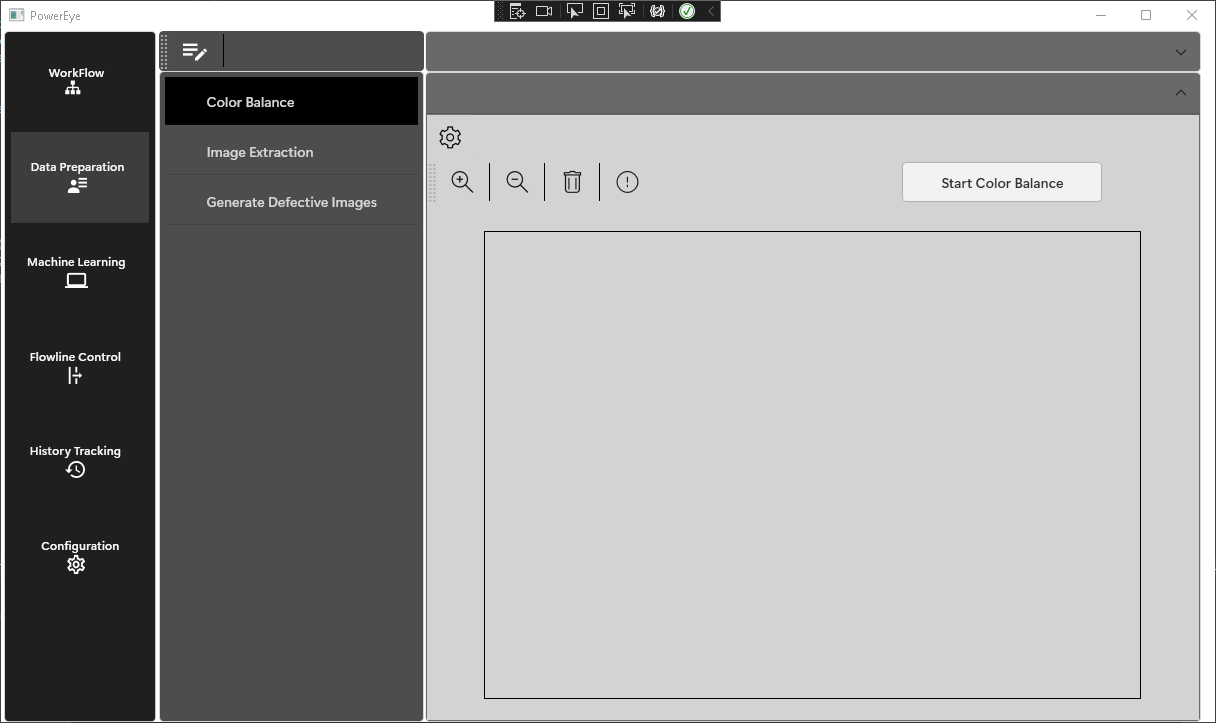
\includegraphics[height=6cm]{ressources/images/color_balance.png}
    \caption{Interface PowerEye redessinée}
\end{figure}
Il contient cinq modules : 
\begin{itemize}
    \item \textbf{Préparation des données (Data preparation): }Ce module permet d'extraire les contours des pièces de l'image et d'ajouter du bruit de perlin à l'image. 
    \item \textbf{Apprentissage automatique (machine learning): }Ce module est utilisé pour entraîner le modèle ckpt à partir de l'ensemble de données.
    \item \textbf{Contrôle de la chaîne d'assemblage (flowline control): } Ce module détecte si une pièce est qualifiée par Template Matching, et enregistre les données du résultat du test.
    \item \textbf{Interroger les données historiques  (History tracking): }Ce module interroge les données du fichier Excel par mots-clés.
    \item \textbf{Configuration des données globales (configuration): }Ce module affiche la configuration complète du logiciel en cours et l'importe par l'intermédiaire de fichiers de configuration.
\end{itemize}